\documentclass[border=4pt]{standalone}
\usepackage{lmodern}
\usepackage{amsmath,amssymb}
\usepackage{pgfplots}
\pgfplotsset{compat=1.18}
\begin{document}
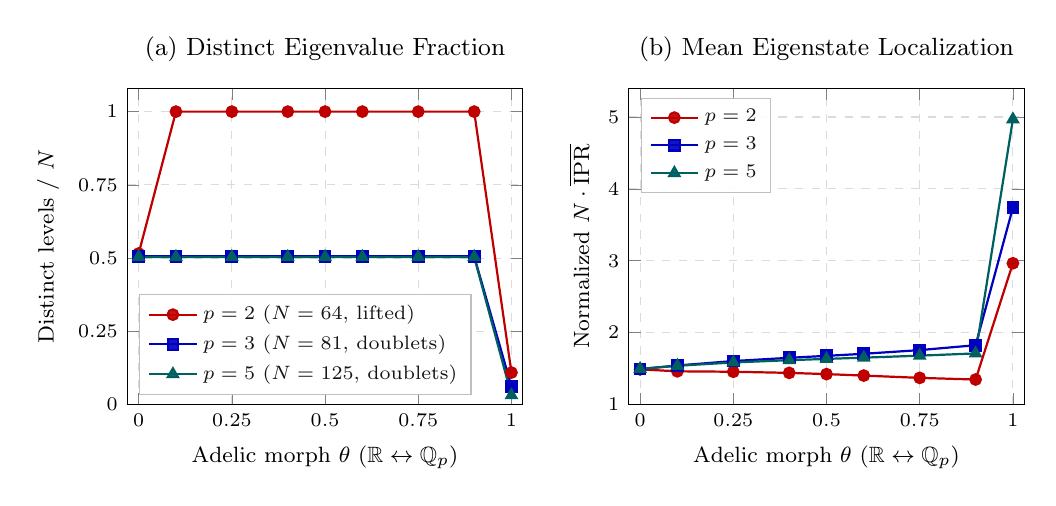
\begin{tikzpicture}
\begin{axis}[
  name=leftplot,
  width=6.6cm,
  height=5.6cm,
  title={\small (a) Distinct Eigenvalue Fraction},
  xlabel={Adelic morph $\theta$ ($\mathbb{R} \leftrightarrow \mathbb{Q}_p$)},
  ylabel={Distinct levels / $N$},
  xmin=-0.03, xmax=1.03,
  ymin=0.0, ymax=1.08,
  xtick={0,0.25,0.5,0.75,1.0},
  ytick={0,0.25,0.5,0.75,1.0},
  grid=major,
  grid style={dashed, gray!28},
  legend pos=south west,
  legend cell align=left,
  legend style={font=\scriptsize, fill=white, fill opacity=0.92, draw=gray!50},
  label style={font=\footnotesize},
  tick label style={font=\scriptsize},
]
  \addplot[color=red!75!black, thick, mark=*, mark size=1.9pt] coordinates { (0.00, 0.51562) (0.10, 1.00000) (0.25, 1.00000) (0.40, 1.00000) (0.50, 1.00000) (0.60, 1.00000) (0.75, 1.00000) (0.90, 1.00000) (1.00, 0.10938) };
  \addlegendentry{$p=2$ ($N=64$, lifted)}
  \addplot[color=blue!75!black, thick, mark=square*, mark size=1.9pt] coordinates { (0.00, 0.50617) (0.10, 0.50617) (0.25, 0.50617) (0.40, 0.50617) (0.50, 0.50617) (0.60, 0.50617) (0.75, 0.50617) (0.90, 0.50617) (1.00, 0.06173) };
  \addlegendentry{$p=3$ ($N=81$, doublets)}
  \addplot[color=teal!75!black, thick, mark=triangle*, mark size=2.1pt] coordinates { (0.00, 0.50400) (0.10, 0.50400) (0.25, 0.50400) (0.40, 0.50400) (0.50, 0.50400) (0.60, 0.50400) (0.75, 0.50400) (0.90, 0.50400) (1.00, 0.03200) };
  \addlegendentry{$p=5$ ($N=125$, doublets)}
\end{axis}

\begin{axis}[
  at={(leftplot.east)},
  anchor=west,
  xshift=1.35cm,
  width=6.6cm,
  height=5.6cm,
  title={\small (b) Mean Eigenstate Localization},
  xlabel={Adelic morph $\theta$ ($\mathbb{R} \leftrightarrow \mathbb{Q}_p$)},
  ylabel={Normalized $N \cdot \overline{\mathrm{IPR}}$},
  xmin=-0.03, xmax=1.03,
  ymin=1.0, ymax=5.4,
  xtick={0,0.25,0.5,0.75,1.0},
  grid=major,
  grid style={dashed, gray!28},
  legend pos=north west,
  legend cell align=left,
  legend style={font=\scriptsize, fill=white, fill opacity=0.92, draw=gray!50},
  label style={font=\footnotesize},
  tick label style={font=\scriptsize},
]
  \addplot[color=red!75!black, thick, mark=*, mark size=1.9pt] coordinates { (0.00, 1.4898) (0.10, 1.4627) (0.25, 1.4567) (0.40, 1.4410) (0.50, 1.4238) (0.60, 1.4033) (0.75, 1.3716) (0.90, 1.3484) (1.00, 2.9651) };
  \addlegendentry{$p=2$}
  \addplot[color=blue!75!black, thick, mark=square*, mark size=1.9pt] coordinates { (0.00, 1.4938) (0.10, 1.5437) (0.25, 1.6054) (0.40, 1.6505) (0.50, 1.6778) (0.60, 1.7065) (0.75, 1.7576) (0.90, 1.8259) (1.00, 3.7385) };
  \addlegendentry{$p=3$}
  \addplot[color=teal!75!black, thick, mark=triangle*, mark size=2.1pt] coordinates { (0.00, 1.4960) (0.10, 1.5398) (0.25, 1.5859) (0.40, 1.6175) (0.50, 1.6354) (0.60, 1.6528) (0.75, 1.6803) (0.90, 1.7118) (1.00, 4.9670) };
  \addlegendentry{$p=5$}
\end{axis}
\end{tikzpicture}
\end{document}
